\documentclass[8pt]{article}
\usepackage[margin=1in]{geometry}
\usepackage{amsmath,amssymb}
\usepackage{graphicx}
\usepackage{listings}
\usepackage{xcolor}
\usepackage{tikz}
\usepackage{tcolorbox}
\usepackage{hyperref}

% Colors
\definecolor{codegreen}{rgb}{0,0.6,0}
\definecolor{codegray}{rgb}{0.5,0.5,0.5}
\definecolor{codepurple}{rgb}{0.58,0,0.82}
\definecolor{backcolour}{rgb}{0.95,0.95,0.92}

% Code style
\lstdefinestyle{mystyle}{
    backgroundcolor=\color{backcolour},   
    commentstyle=\color{codegreen},
    keywordstyle=\color{magenta},
    numberstyle=\tiny\color{codegray},
    stringstyle=\color{codepurple},
    basicstyle=\ttfamily\footnotesize,
    breakatwhitespace=false,         
    breaklines=true,                 
    captionpos=b,                    
    keepspaces=true,                 
    numbers=left,                    
    numbersep=5pt,                  
    showspaces=false,                
    showstringspaces=false,
    showtabs=false,                  
    tabsize=2
}
\lstset{style=mystyle}

% Custom commands
\newcommand{\question}[1]{\vspace{0.5em}\noindent\textbf{Q: #1}\vspace{0.3em}}
\newcommand{\exercise}[1]{\vspace{0.5em}\noindent\textbf{Exercise: #1}\vspace{0.3em}}
\newcommand{\think}[1]{\vspace{0.3em}\noindent\textit{Think: #1}\vspace{0.3em}}
\newcommand{\discovery}[1]{
    \begin{tcolorbox}[colback=green!5!white,colframe=green!75!black,title=Discovery]
    #1
    \end{tcolorbox}
}

\title{Week 4: Teaching Machines to Translate\\
\large Discovery-Based Learning Exercises (Student Version)}
\date{}

\begin{document}
\maketitle

\section*{Learning Objectives}
By the end of this session, you will:
\begin{itemize}
    \item Discover why variable-length input/output is challenging
    \item Design your own encoder-decoder architecture
    \item Identify the information bottleneck problem
    \item Invent the attention mechanism
\end{itemize}

\hrule
\vspace{1em}

\section{Part 1: The Translation Challenge (10 minutes)}

\subsection{Warm-up: Word-by-Word Translation}

\question{Let's try translating English to French word-by-word:}

\begin{center}
\begin{tabular}{|l|l|}
\hline
\textbf{English} & \textbf{French (word-by-word)} \\
\hline
The cat sat on the mat & Le chat \_\_\_ sur le tapis \\
How are you? & Comment \_\_\_ \_\_\_? \\
I love natural language processing & Je \_\_\_ naturel langue traitement \\
\hline
\end{tabular}
\end{center}

\vspace{2em} % Space for student answers

\question{What problems do you notice with word-by-word translation?}

\vspace{3em} % Space for student answers

\subsection{The Length Mismatch Problem}

\exercise{Count the words in these equivalent sentences:}

\begin{itemize}
    \item English: "I love you" = \_\_\_ words
    \item French: "Je t'aime" = \_\_\_ words  
    \item German: "Ich liebe dich" = \_\_\_ words
    \item Japanese (romanized): "Aishiteru" = \_\_\_ word(s)
\end{itemize}

\think{If a neural network produces one output per input, how can it handle these different lengths?}

\vspace{3em} % Space for student reflection

\subsection{Design Challenge}

\question{You're building a translation system. Your input is a sequence of English words, your output needs to be French words. The lengths don't match. How would YOU solve this?}

Draw your solution here:

\vspace{8em} % Space for student drawing

\discovery{
If you thought of processing the entire input first before generating output, you're thinking like a sequence-to-sequence model designer!
}

\section{Part 2: Building the Bridge (15 minutes)}

\subsection{The Compression Exercise}

\exercise{Compress these sentences into exactly 3 numbers, then try to reconstruct them:}

\begin{enumerate}
    \item "The cat sat" $\rightarrow$ [\_\_\_, \_\_\_, \_\_\_]
    \item "A dog ran quickly" $\rightarrow$ [\_\_\_, \_\_\_, \_\_\_]
    \item "The International Conference on Machine Learning accepted our paper about neural networks" $\rightarrow$ [\_\_\_, \_\_\_, \_\_\_]
\end{enumerate}

\question{Which sentence was hardest to compress? Why?}

\vspace{3em} % Space for answer

\question{Which information did you lose in sentence 3?}

\vspace{3em} % Space for answer

\subsection{The Two-Network Solution}

\think{What if we had TWO separate networks - one to read/understand, one to write/generate?}

Fill in this diagram with what each network should do:

\begin{center}
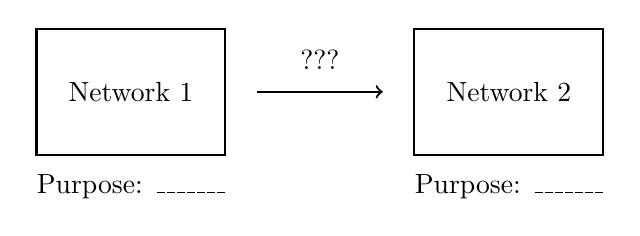
\begin{tikzpicture}[scale=0.8]
    % First network
    \draw[thick] (0,0) rectangle (3,2);
    \node at (1.5,1) {Network 1};
    \node at (1.5,-0.5) {Purpose: \_\_\_\_\_\_\_};
    
    % Arrow
    \draw[->, thick] (3.5,1) -- (5.5,1);
    \node at (4.5,1.5) {???};
    
    % Second network  
    \draw[thick] (6,0) rectangle (9,2);
    \node at (7.5,1) {Network 2};
    \node at (7.5,-0.5) {Purpose: \_\_\_\_\_\_\_};
\end{tikzpicture}
\end{center}

\question{What should pass between the two networks (what goes in the ??? box)?}

\vspace{3em} % Space for answer

\discovery{
Congratulations! You just invented the encoder-decoder architecture! 
Network 1 = Encoder (compresses input to understanding)
Network 2 = Decoder (generates output from understanding)
}

\section{Part 3: The Bottleneck Discovery (10 minutes)}

\subsection{Long Sentence Challenge}

\exercise{Try to translate this paragraph using your two-network system:}

\begin{tcolorbox}[colback=blue!5!white]
"The International Conference on Machine Learning, which is one of the premier venues for presenting research in machine learning and attracts submissions from researchers around the world working on various aspects of learning algorithms, accepted our paper about using neural networks for natural language understanding, specifically focusing on how attention mechanisms can improve translation quality."
\end{tcolorbox}

\question{If you compress this entire paragraph into a fixed-size vector (say, 256 numbers), what information might you lose?}

\begin{itemize}
    \item Beginning: \_\_\_\_\_\_\_\_\_\_\_\_\_
    \item Middle: \_\_\_\_\_\_\_\_\_\_\_\_\_
    \item End: \_\_\_\_\_\_\_\_\_\_\_\_\_
\end{itemize}

\think{This is like trying to remember an entire book by storing it as a single "feeling" - you'll forget the details!}

\subsection{Information Theory}

\question{Calculate the information loss:}

\begin{itemize}
    \item Short sentence (5 words) compressed to 256 numbers: \underline{Minimal} loss
    \item Long document (500 words) compressed to 256 numbers: \underline{\_\_\_\_\_} loss
\end{itemize}

\question{What's the fundamental problem here?}

\vspace{3em} % Space for answer

\discovery{
You've identified the information bottleneck! Fixed-size representations can't capture all the information from arbitrarily long sequences.
}

\section{Part 4: Inventing Attention (15 minutes)}

\subsection{Human Translation Process}

\exercise{Translate this sentence step by step, marking which English words you look at for each French word:}

English: "The black cat sat on the mat"

\begin{center}
\begin{tabular}{|l|l|}
\hline
\textbf{Generating French word} & \textbf{Looking at English words} \\
\hline
"Le" & \_\_\_\_\_\_\_\_\_\_\_ \\
"chat" & \_\_\_\_\_\_\_\_\_\_\_ \\
"noir" & \_\_\_\_\_\_\_\_\_\_\_ \\
"s'est assis" & \_\_\_\_\_\_\_\_\_\_\_ \\
"sur" & \_\_\_\_\_\_\_\_\_\_\_ \\
"le" & \_\_\_\_\_\_\_\_\_\_\_ \\
"tapis" & \_\_\_\_\_\_\_\_\_\_\_ \\
\hline
\end{tabular}
\end{center}

\think{Notice how you don't look at ALL words equally - you focus on relevant parts!}

\subsection{Designing the Looking-Back Mechanism}

\question{Instead of compressing everything into one vector, what if the decoder could "look back" at all encoder states? Design a mechanism:}

\begin{enumerate}
    \item How would you decide which encoder states are relevant? \\
    \vspace{2em}
    
    \item How would you combine multiple relevant states? \\
    \vspace{2em}
    
    \item How would you turn this into weights that sum to 1? \\
    \vspace{2em}
\end{enumerate}

\subsection{Computing Attention Scores}

\exercise{For the word "chat" (cat), assign relevance scores (0-1) to each English word:}

\begin{center}
\begin{tabular}{|l|c|}
\hline
\textbf{English word} & \textbf{Relevance to "chat"} \\
\hline
The & \_\_\_ \\
black & \_\_\_ \\
cat & \_\_\_ \\
sat & \_\_\_ \\
on & \_\_\_ \\
the & \_\_\_ \\
mat & \_\_\_ \\
\hline
\textbf{Total} & Should sum to 1.0 \\
\hline
\end{tabular}
\end{center}

\discovery{
You just invented attention! Your relevance scores are attention weights, and looking back at all encoder states based on relevance is exactly how attention works!
}

\section{Part 5: Putting It All Together (10 minutes)}

\subsection{Complete Architecture}

Draw the complete sequence-to-sequence model with attention:

\vspace{10em} % Space for drawing

\subsection{Key Components Checklist}

Check off each component you included:
\begin{itemize}
    \item[$\square$] Encoder network (processes input)
    \item[$\square$] Multiple encoder hidden states (not just final)
    \item[$\square$] Decoder network (generates output)
    \item[$\square$] Attention mechanism (looks back at encoder states)
    \item[$\square$] Attention weights (relevance scores)
    \item[$\square$] Context vector (weighted sum)
\end{itemize}

\subsection{Reflection Questions}

\question{Why is attention better than a fixed-size bottleneck?}

\vspace{3em}

\question{What tasks besides translation could benefit from this architecture?}

\vspace{3em}

\question{What limitations might this approach still have?}

\vspace{3em}

\section{Bonus Challenge: Beam Search}

\think{When generating translations, should we always pick the most likely next word?}

\exercise{Consider translating "bank" - it could mean financial institution or river bank. Design a strategy to explore multiple translation paths:}

\vspace{5em}

\hrule
\vspace{1em}

\section*{Summary}

Today you discovered:
\begin{enumerate}
    \item The variable-length challenge in translation
    \item The encoder-decoder architecture
    \item The information bottleneck problem
    \item The attention mechanism
\end{enumerate}

These concepts you "invented" are the foundation of modern machine translation systems like Google Translate!

\vspace{2em}
\noindent\textbf{Next Week:} We'll see how taking attention to the extreme (attention is ALL you need) leads to Transformers!

\end{document}